\documentclass[aspectratio=169, table]{beamer}

\usepackage{colortbl}
\usepackage{xcolor}
\usepackage{listings}
\usepackage{tikz}
\usetikzlibrary{positioning, arrows.meta, fit}

\usetheme{Pradita}


\usepackage{listings}
\lstdefinestyle{SqlStyle}{
language=SQL,
basicstyle=\ttfamily\footnotesize,
morekeywords={REAL, TEXT, REFERENCES},
keywordstyle=\color{blue},
commentstyle=\color{gray},
stringstyle=\color{red},
breaklines=true,
showstringspaces=false,
tabsize=2,
captionpos=b,
numbers=left,
numberstyle=\tiny\color{gray},
frame=lines,
backgroundcolor=\color{lightgray!10},
comment=[l]{//},
morecomment=[s]{/*}{*/},
commentstyle=\color{gray}\ttfamily,
string=[s]{'}{'},
morestring=[s]{"}{"},
%	stringstyle=\color{teal}\ttfamily,
%	showstringspaces=false
}

\lstdefinelanguage{bash} {
keywords={},
basicstyle=\ttfamily\small,
keywordstyle=\color{blue}\bfseries,
ndkeywords={iex},
ndkeywordstyle=\color{purple}\bfseries,
sensitive=true,
commentstyle=\color{gray},
stringstyle=\color{red},
numbers=left,
numberstyle=\tiny\color{gray},
breaklines=true,
frame=lines,
backgroundcolor=\color{lightgray!10},
tabsize=2,
comment=[l]{\#},
morecomment=[s]{/*}{*/},
commentstyle=\color{gray}\ttfamily,
stringstyle=\color{purple}\ttfamily,
showstringspaces=false
}


\title{\Huge Understanding\\
\vspace{10pt}
Database and Query}
\subtitle{IT140704 - Big Data for Business}
%\date[Serial]{Penggunaan Large Language Model untuk Pengajaran}
\author{\textbf{Alfa Yohannis}}
\begin{document}

\frame{\titlepage}


\begin{frame}[fragile]
\frametitle{Contents}
\vspace{20pt}
\begin{columns}[t]
	\column{0.5\textwidth}
	\tableofcontents[sections={1-4}]
	
	\column{0.5\textwidth}
	\tableofcontents[sections={5-8}]
\end{columns}
\end{frame}


\begin{frame}{\hfill}
\centering
\Huge{\textbf{How is data structured, managed, and queried to support business decisions in the era of big data?}}
\end{frame}


\section{Structured Data Management}

\begin{frame}[fragile]{Managing Structured Data}
\vspace{20pt}

Effective data management begins with understanding how data is stored. \textbf{Relational databases} provide a dominant approach to storing, organizing, and quickly accessing structured data. This concept—alongside the role of \textbf{SQL}—forms the foundation for building information systems, answering business questions, and integrating into \emph{big data} architectures.\\[12pt]

\begin{columns}[T]
\column{0.48\textwidth}
\textbf{What is Structured Data?}
\begin{itemize}
	\item Fixed schema (rows–columns).
	\item \emph{Self-describing}: primary and foreign keys.
	\item Supports integration and quality control.
\end{itemize}

\column{0.52\textwidth}
\textbf{Role in the Big Data Era}
\begin{itemize}
	\item Most mature in terms of governance.
	\item Dominates the \emph{curated zone} of data warehouses.
	\item SQL is supported by modern parallel engines.
\end{itemize}
\end{columns}

\end{frame}

\begin{frame}[fragile]{A Brief History of Relational Databases}
\vspace{20pt}

\begin{itemize}
\item \textbf{1960s} – Era of \textit{hierarchical} and \textit{network models}.  
Early example: Integrated Data Store (IDS) at General Electric.

\item \textbf{1970} – Edgar F. Codd published the concept of the \emph{Relational Model};  
two-dimensional tables (\textit{relations}) and relational logic replaced pointer navigation.

\item \textbf{1974–1978} – IBM's \textit{System R} became the first research implementation  
and introduced the \textbf{SQL} language.

\item \textbf{1979–1980s} – Commercial products emerged: Oracle, Informix, Sybase,  
Microsoft SQL Server; SQL was standardized as ANSI SQL (1986).

\item \textbf{1990s–present} – Relational databases remain foundational, evolving toward  
large-scale processing (MPP), emerging NoSQL/NewSQL systems, and integration with  
\textit{big data} architectures.
\end{itemize}

\end{frame}

\section{Understanding Structured Data in Tables}

\begin{frame}[fragile]{Structured Data Example: \texttt{orders.csv}}
\vspace{20pt}

Order data in transactional systems is often stored in \texttt{.csv} format to support easy integration with relational database systems (RDBMS). This file represents an \emph{Order} entity and includes key attributes for supporting business processes such as transaction tracking, revenue calculation, and customer performance analysis.

\begin{columns}[T,onlytextwidth]

\column{0.58\textwidth}
\begin{lstlisting}[language=bash, caption={file \texttt{orders.csv}}, basicstyle=\ttfamily\scriptsize, label={lst:orders_csv}]
	id,customer_id,date,total
	201,1,2024-01-12,15000000
	202,2,2024-01-15,8502000
	203,1,2024-01-18,45000
	204,3,2024-02-01,130000
	205,4,2024-02-10,68000
\end{lstlisting}

\column{0.42\textwidth}
\begin{itemize}
	\item \texttt{id}: unique order identifier  
	\item \texttt{customer\_id}: relation to customer  
	\item \texttt{date}: transaction date  
	\item \texttt{total}: total order value  
\end{itemize}

\end{columns}

This structure enables SQL queries such as monthly sales aggregation, identification of active customers, and sales performance reporting in modern analytics systems.

\end{frame}

\begin{frame}[fragile]{Structured Data Example: \texttt{customers.csv}}
\vspace{20pt}

Customer data is recorded in structured formats such as \texttt{.csv} for efficient management in relational database systems. This file represents a \emph{Customer} entity and is used for various business analyses such as customer segmentation and tracking regional contributions to sales.

\begin{columns}[T,onlytextwidth]

\column{0.58\textwidth}
\begin{lstlisting}[language=bash, caption={file \texttt{customers.csv}}, basicstyle=\ttfamily\scriptsize, label={lst:customers_csv}]
	id,name,city
	1,Andi Surya,Jakarta
	2,Budi Santoso,Bandung
	3,Citra Lestari,Surabaya
	4,Dewi Anggraini,Medan
	5,Eko Prasetyo,Yogyakarta
	6,Fitri Aulia,Semarang
\end{lstlisting}

\column{0.42\textwidth}
\begin{itemize}
	\item \texttt{id}: customer primary key  
	\item \texttt{name}: full name  
	\item \texttt{city}: city of residence  
\end{itemize}

\end{columns}

This file is a key reference in one-to-many relationships with the \texttt{orders} table, enabling integrated analysis between customer and transactional data.

\end{frame}

\begin{frame}[fragile]{Tables, Columns, Rows, and Key Relationships}
\vspace{15pt}

The relational model stores data in two-dimensional \textbf{tables} representing entities such as customers or transactions.  
This structure supports both efficiency and data integrity.

\begin{columns}[T]

\column{0.5\textwidth}
\textbf{Table Structure}
\begin{itemize}
	\item \textbf{Columns (attributes)} — data types, e.g., \texttt{name}, \texttt{price}
	\item \textbf{Rows (tuples)} — one real instance of an entity
\end{itemize}

\textbf{Types of Keys}
\begin{itemize}
	\item \textbf{Primary Key} — unique, non-null, identifies each row
	\item \textbf{Foreign Key} — references the \emph{Primary Key} in another table
\end{itemize}

\column{0.5\textwidth}
\textbf{Relationship Examples}
\begin{itemize}
	\item \texttt{orders.customer\_id} $\rightarrow$ \texttt{customers.id}
	\item \texttt{order\_details.order\_id} $\rightarrow$ \texttt{orders.id}
\end{itemize}

\textbf{Benefits of Relationships}
\begin{itemize}
	\item Supports table \textbf{JOINs}
	\item Minimises data duplication (normalisation)
	\item Simplifies validation and maintenance
\end{itemize}

\end{columns}

\end{frame}


\section{Relational Data Model and Practice Tools}

\begin{frame}{Entity Relationship Diagram (1)}
\vspace{20pt}

The relational data structure in an e-commerce context typically involves four key entities:

\begin{itemize}
\item \textbf{Customer} – stores customer details such as \texttt{id}, \texttt{name}, and \texttt{city}.
\item \textbf{Order} – represents purchase transactions, with attributes including \texttt{id}, \texttt{customer\_id}, \texttt{date}, and \texttt{total}.
\item \textbf{OrderDetail} – describes individual items within each order, including \texttt{order\_id}, \texttt{product\_id}, and \texttt{quantity}.
\item \textbf{Product} – holds product information such as \texttt{id}, \texttt{name}, \texttt{category}, and \texttt{price}.
\end{itemize}

These entity relationships are commonly applied in point-of-sale systems, ERP software, and e-commerce applications.

\end{frame}

\begin{frame}{Entity Relationship Diagram (2)}
\vspace{20pt}

\begin{figure}
\centering
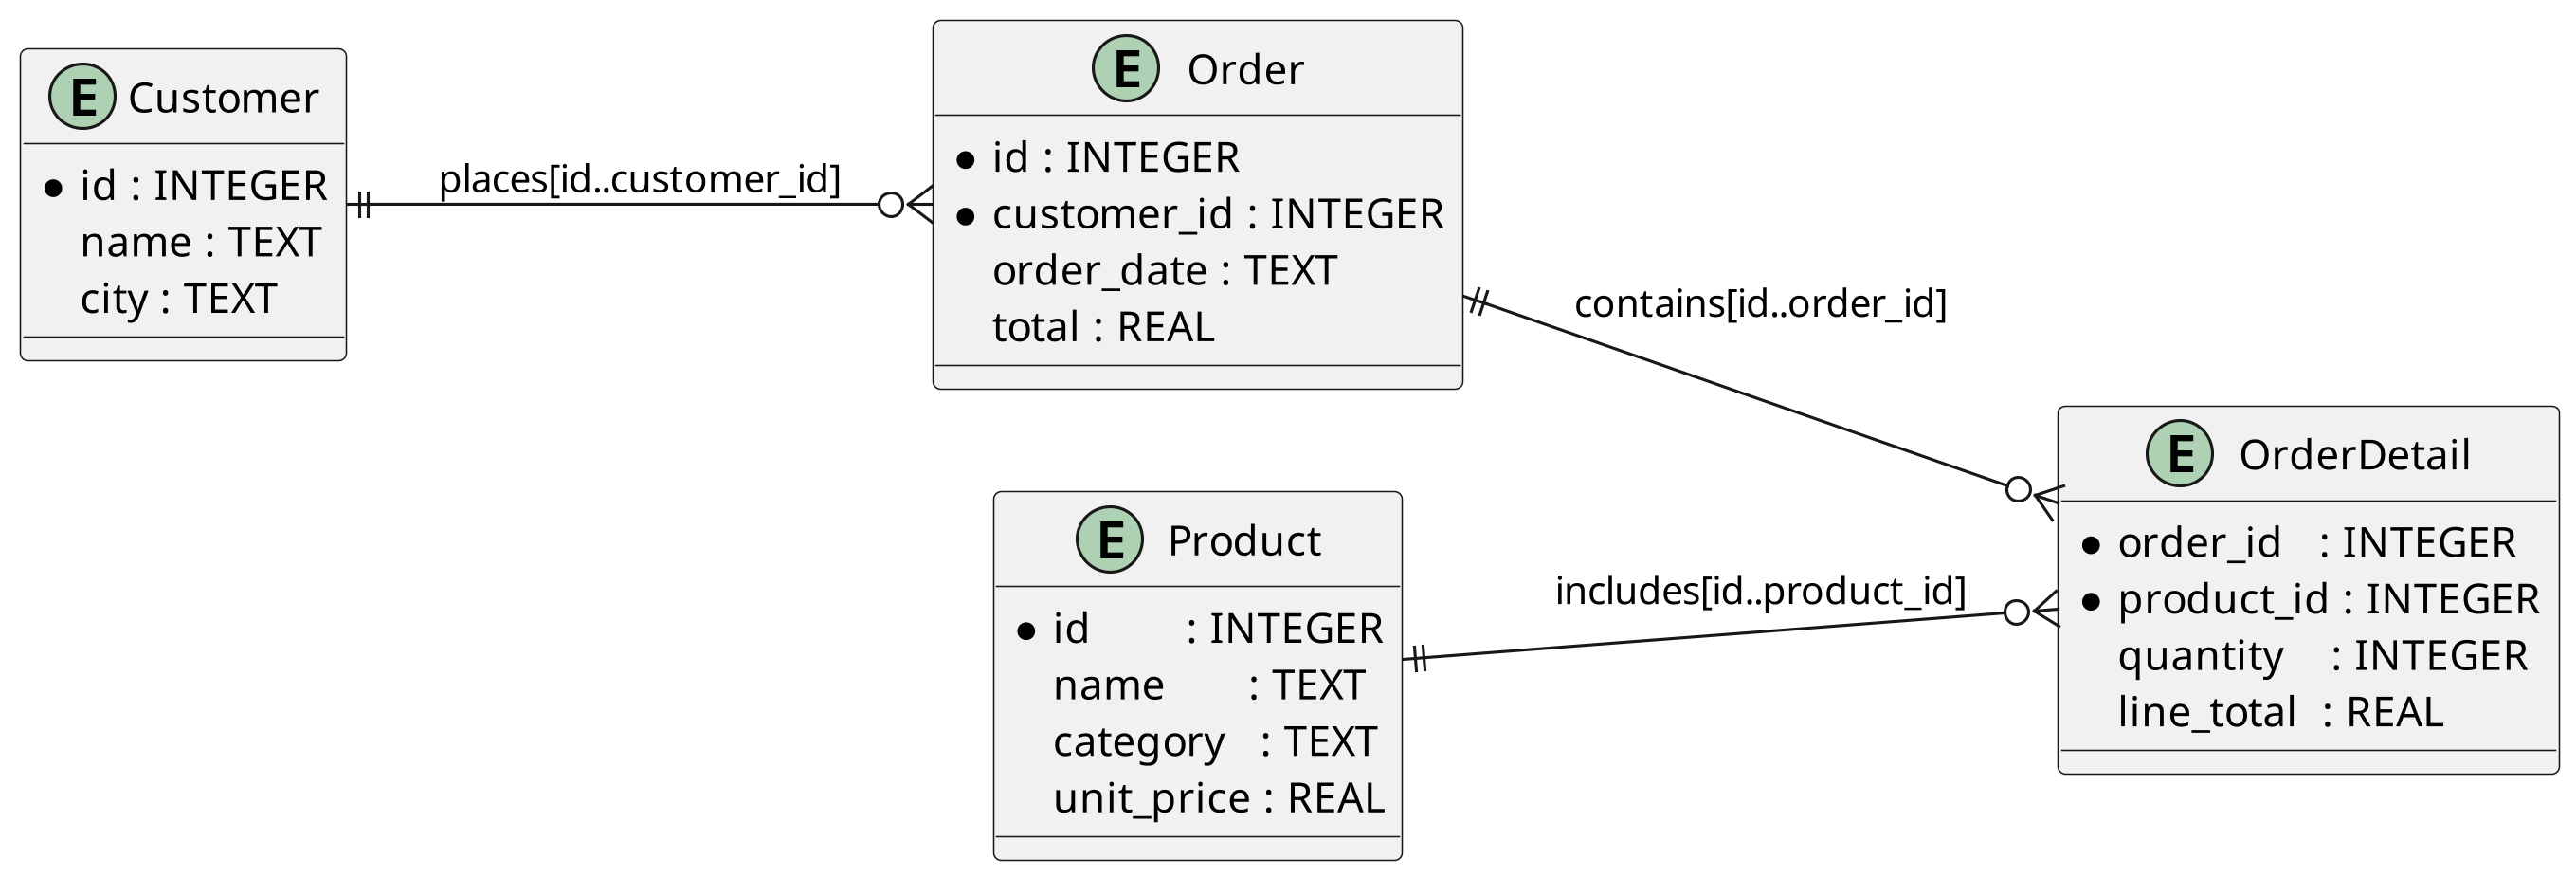
\includegraphics[width=\textwidth]{data/out/erd.png}
\label{fig:customer_order_erd}
\end{figure}

\vspace{-30pt}
\begin{itemize}
\item \texttt{orders.customer\_id} $\rightarrow$ \texttt{customers.id}
\item \texttt{order\_details.order\_id} $\rightarrow$ \texttt{orders.id}
\item \texttt{order\_details.product\_id} $\rightarrow$ \texttt{products.id}
\end{itemize}

\end{frame}

\begin{frame}{Practice Tools: DB Browser and SQLite}
\vspace{20pt}

\textbf{SQLite} is a lightweight relational database management system that does not require a separate server. All data is stored in a single local file, making it ideal for mobile apps, embedded systems, and educational purposes.

\vspace{10pt}
To support hands-on practice without complex server installation, \textbf{DB Browser for SQLite} is used—a lightweight graphical interface for creating, editing, and running SQL queries on SQLite databases.

\vspace{10pt}
DB Browser is well-suited for learning environments due to:
\begin{itemize}
\item Free and open-source availability
\item Lightweight setup, no server configuration required
\item Features such as drag-and-drop, table visualisation, and interactive SQL editor
\end{itemize}

\end{frame}

\begin{frame}{DB Browser for SQLite Interface}
\vspace{20pt}

\begin{figure}
\centering
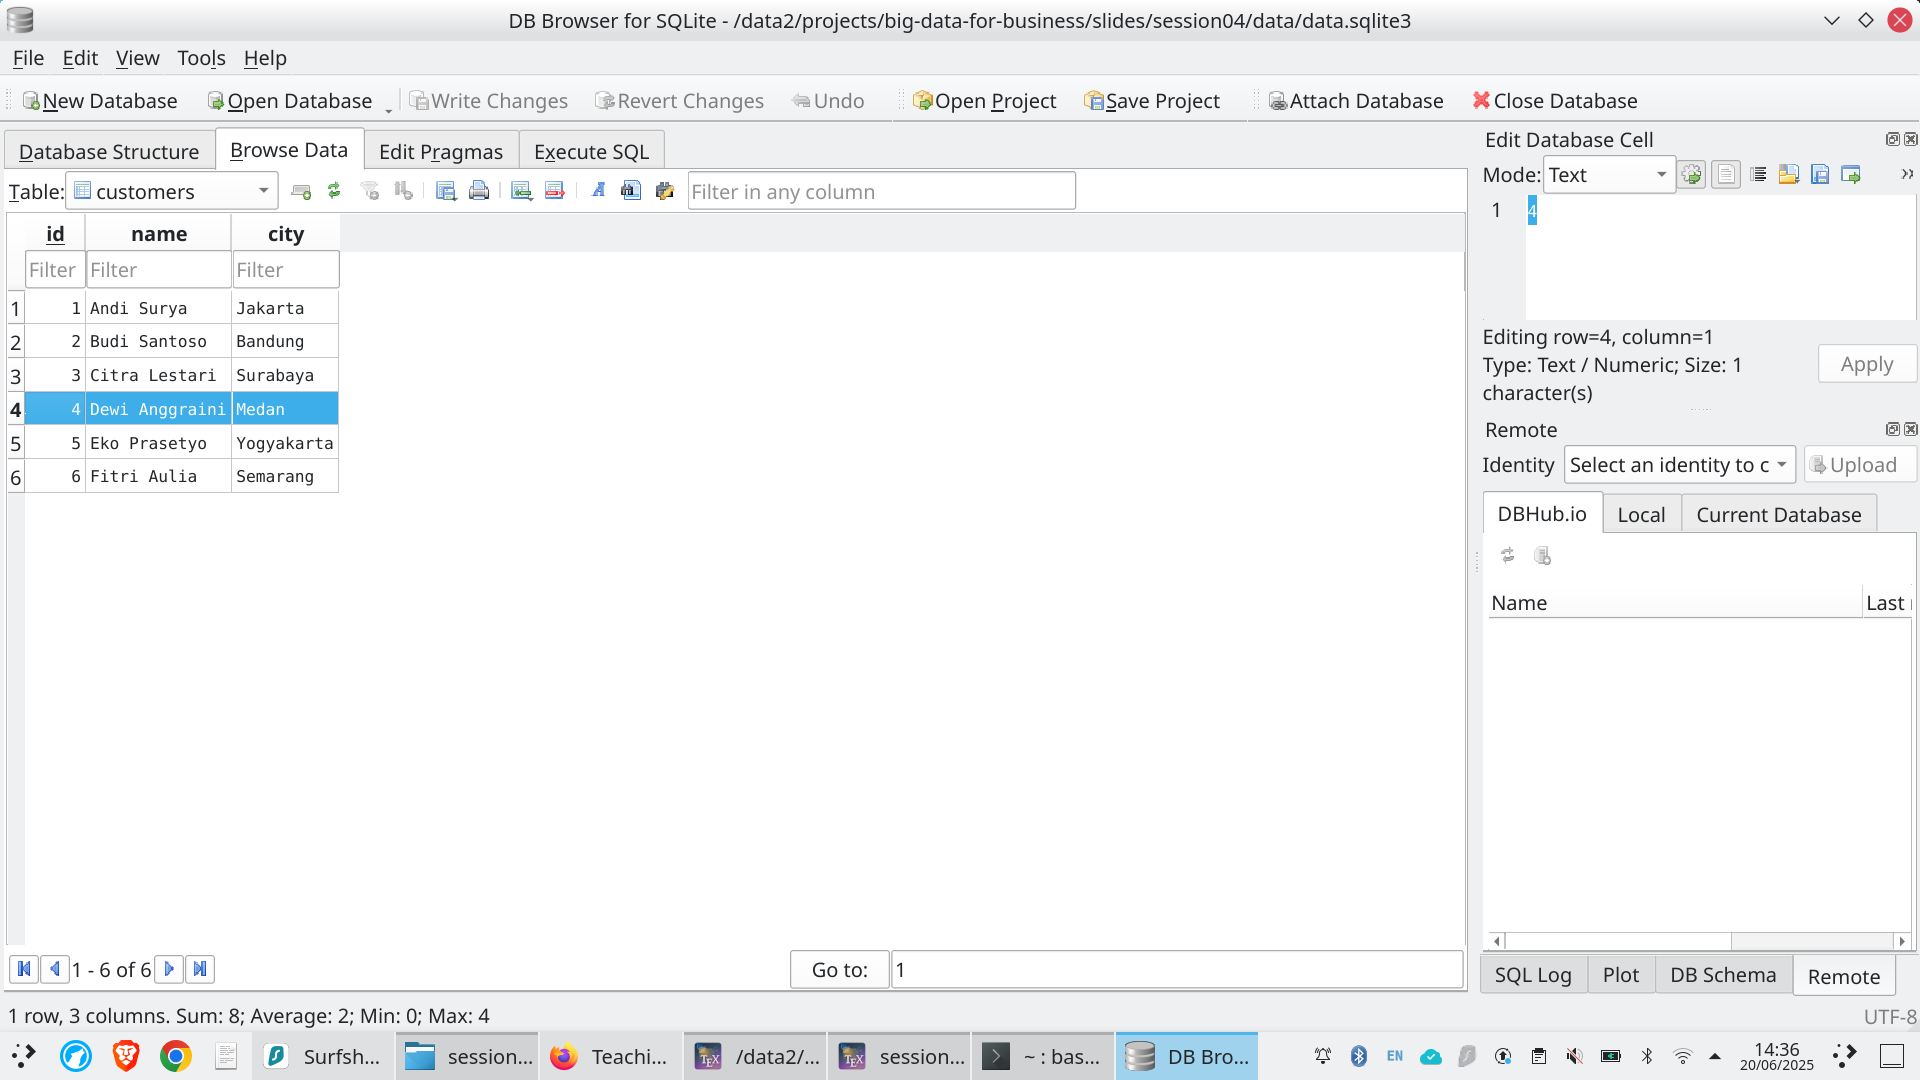
\includegraphics[width=.8\textwidth]{../../figures/dbbrowser.png}
\label{fig:dbbrowser}
\end{figure}

\end{frame}



\section{Getting Started with DB Browser and SQL Queries}

\begin{frame}{Installing DB Browser for SQLite}
\vspace{20pt}

The following steps apply to Windows, macOS, and Linux operating systems:

\begin{enumerate}
\item Visit the official site: \url{https://sqlitebrowser.org}
\item Click on the \textbf{Download} menu, then choose the installer appropriate for your OS:
\begin{itemize}
	\item Windows: \texttt{Standard installer for 64-bit Windows}
	\item macOS: \texttt{DB Browser for SQLite.dmg}
	\item Linux (Ubuntu): run the terminal command \texttt{sudo apt install sqlitebrowser}
\end{itemize}
\item Follow the installation instructions provided for your system.
\end{enumerate}
\end{frame}

\begin{frame}[fragile]{Initial Hands-on with DB Browser}
\vspace{20pt}

\begin{columns}[T,onlytextwidth]
%-------------------------%
\column{0.55\textwidth}
\begin{enumerate}
	\item Open the database file \textbf{data.sqlite3}.
	\item Click the \textbf{Database Structure} tab to view table schemas and relationships. Right-click a table and choose \textbf{Modify Table}.
	\item Switch to the \textbf{Browse Data} tab to inspect records. Select \texttt{order\_details} from the combo box, try editing a \texttt{quantity} value.
	\item Run simple SQL queries in the \textbf{Execute SQL} tab.
\end{enumerate}

%-------------------------%
\column{0.4\textwidth}
\begin{lstlisting}[style=SqlStyle]
	-- First 5 customers
	SELECT * FROM customer 
	LIMIT 5;
	
	-- Unique customer cities
	SELECT DISTINCT city 
	FROM customer;
	
	-- Total order value per customer
	SELECT customer_id, 
	SUM(total)
	FROM orders
	GROUP BY customer_id;
\end{lstlisting}

\end{columns}
\end{frame}

\section{Answering 3 Business Questions}
\begin{frame}[fragile]{Sales Insights (1): Customers Without Orders}
\vspace{20pt}

\textbf{Business Question:} Which customers have never placed an order?

\begin{lstlisting}[style=SqlStyle]
SELECT c.name FROM customers c
LEFT JOIN orders o ON c.id = o.customer_id
WHERE o.id IS NULL;
\end{lstlisting}

Explanation:
\begin{itemize}
\item \texttt{LEFT JOIN} includes all customers, even those without orders.
\item \texttt{WHERE o.id IS NULL} filters to show only customers with no transactions.
\end{itemize}
\end{frame}

\begin{frame}[fragile]{Sales Insights (2): Top Cities by Revenue}
\vspace{20pt}

\textbf{Business Question:} Which cities generate the highest sales?

\begin{lstlisting}[style=SqlStyle]
SELECT c.city, SUM(o.total) AS total_sales
FROM customers c
JOIN orders o ON c.id = o.customer_id
GROUP BY c.city
ORDER BY total_sales DESC
LIMIT 5;
\end{lstlisting}

This query aggregates customer and order data, groups by city, sorts by revenue, and returns the top 5.

\end{frame}

\begin{frame}[fragile]{GROUP BY and Aggregate Functions}
\vspace{20pt}

\textbf{Business Question:} Which product categories contribute the most revenue?

\begin{lstlisting}[style=SqlStyle]
SELECT p.category, SUM(od.line_total) AS total_revenue
FROM order_details od
JOIN products p ON p.id = od.product_id
GROUP BY p.category
ORDER BY total_revenue DESC;
\end{lstlisting}

The \texttt{SUM} function combined with \texttt{GROUP BY} enables analysis of revenue contribution per product category.

\end{frame}


\section{SQL Query Practice}

\begin{frame}[fragile]{Exercise: Answering Business Questions}
\vspace{20pt}

Independent SQL exploration challenge:

\begin{enumerate}
\item Which product is most frequently purchased?
\item Which customer contributes the highest total sales?
\item What is the average transaction value per city?
\item Are there any products that have never been sold?
\end{enumerate}

Example: Most frequently purchased product

\begin{lstlisting}[style=SqlStyle]
SELECT p.name, SUM(od.quantity) AS total_quantity
FROM order_details od
JOIN products p ON p.id = od.product_id
GROUP BY p.name
ORDER BY total_quantity DESC
LIMIT 1;
\end{lstlisting}

\end{frame}


\section{Comparison of Popular RDBMS Products}
\begin{frame}{Comparison of Popular RDBMS Products}
\vspace{20pt}

\renewcommand{\arraystretch}{1.3}
{\footnotesize
\arrayrulewidth=0.7pt
\setlength{\tabcolsep}{3pt}
\arrayrulecolor{black}
\begin{tabular}{|p{0.12\textwidth}|p{0.13\textwidth}|p{0.17\textwidth}|p{0.2\textwidth}|p{0.3\textwidth}|}
	\hline
	\textbf{Product} & \textbf{Vendor} & \textbf{License Type} & \textbf{Scalability} & \textbf{Typical Use Cases} \\ \hline
	MySQL      & Oracle              & Open Source / Commercial & Medium–High & Web Apps, CMS \\ \hline
	PostgreSQL & Community           & Open Source              & High        & Data Analytics, ERP \\ \hline
	SQLite     & Community           & Open Source              & Low–Medium  & Mobile, Embedded \\ \hline
	SQL Server & Microsoft           & Commercial               & High        & Enterprise, Finance \\ \hline
	Oracle DB  & Oracle              & Commercial               & Very High   & Banking, Large-scale ERP \\ \hline
	MariaDB    & MariaDB Foundation  & Open Source              & Medium–High & MySQL Replacement, Hosting \\ \hline
\end{tabular}
}
\end{frame}

\begin{frame}{Aspect: Licensing and Cost}
\vspace{20pt}

\begin{itemize}
\item \textbf{Open Source} – PostgreSQL, SQLite, MariaDB  
\begin{itemize}
	\item Free to use and modify; ideal for research and low-cost development.
\end{itemize}
\item \textbf{Commercial} – Oracle DB, Microsoft SQL Server  
\begin{itemize}
	\item Enterprise features (HA, security, support); licensing per CPU, user, or subscription.
\end{itemize}
\item \textbf{Hybrid} – MySQL Community vs. MySQL Enterprise  
\begin{itemize}
	\item Free version plus paid options with SLA and extra features.
\end{itemize}
\end{itemize}

Total Cost of Ownership (TCO), vendor support, and required features should be carefully evaluated when choosing an RDBMS.

\end{frame}

\begin{frame}{Aspect: Performance and Scalability}
\vspace{20pt}

\begin{itemize}
\item \textbf{Query Optimization} – PostgreSQL and Oracle support parallel queries and advanced indexing.
\item \textbf{Vertical vs. Horizontal Scaling}  
\begin{itemize}
	\item SQL Server: Always On, sharding.  
	\item MySQL: replication, clustering (InnoDB Cluster, Galera).
\end{itemize}
\item \textbf{Embedded/Local} – SQLite is fast for single-user apps but not suitable for high-volume OLTP workloads.
\end{itemize}

Performance evaluation factors:
\begin{itemize}
\item Indexing, partitioning, and caching.  
\item Concurrency mechanisms (MVCC, locking).  
\item Join/sub-query performance at large scale.
\end{itemize}

\end{frame}



%================================================
% Frame — Cloud Support and Vendor Lock-in
%================================================
\begin{frame}{Aspect: Cloud Support and Vendor Lock-in}
\vspace{20pt}

\begin{itemize}
\item \textbf{Managed Services}
\begin{itemize}
	\item Amazon RDS — MySQL, PostgreSQL, MariaDB, SQL Server, Oracle  
	\item Google Cloud SQL — MySQL, PostgreSQL  
	\item Azure SQL Database — fully-managed SQL Server
\end{itemize}

\item \textbf{Lock-in Risks}
\begin{itemize}
	\item Dependence on proprietary features and storage formats  
	\item Complex migrations and high exit costs
\end{itemize}
\end{itemize}

\textbf{Mitigation →} adopt open-source, multi-cloud RDBMS options, rely on standard SQL, and build an abstraction layer.
\end{frame}

%================================================
% Frame — Choosing an RDBMS for Business Needs
%================================================
\begin{frame}{Selecting an RDBMS Based on Business Needs}
\vspace{20pt}

\begin{itemize}
\item \textbf{Data volume \& type}
\begin{itemize}
	\item Large datasets $\rightarrow$ PostgreSQL / Oracle  
	\item Lightweight apps $\rightarrow$ SQLite / MySQL
\end{itemize}

\item \textbf{Transaction profile} — high concurrency demands strong MVCC (SQL Server, PostgreSQL)

\item \textbf{Ecosystem fit} — Microsoft-centric firms leverage SQL Server; open-source stacks align with PostgreSQL/MariaDB

\item \textbf{Budget} — PostgreSQL \& MariaDB have no licence fees; Oracle offers premium paid features

\item \textbf{Analytics} — PostgreSQL + TimescaleDB for time-series, or graph extensions
\end{itemize}

Evaluating these factors leads to rational, sustainable technology choices.
\end{frame}

%================================================
% Frame — Structured Data, SQL, and Big-Data Architecture
%================================================
\section{Structured Data, SQL, and Big-Data Architecture}
\begin{frame}{Structured Data, SQL, Big-Data Architecture}
\vspace{20pt}

\begin{columns}[T]

%----------- Left Column -----------
\column{0.5\textwidth}
\textbf{Position of Structured Data}
\begin{itemize}
	\item Still critical in the big-data era
	\item Tabular format with fixed schema
	\item Sources: transactions, finance, HR, services
	\item Stored in the \emph{structured zone} of a data lake
	\item Hive, Presto, Impala run SQL on HDFS/S3
\end{itemize}

%----------- Right Column -----------
\column{0.5\textwidth}
\textbf{SQL in the ETL Pipeline}
\begin{itemize}
	\item \textbf{Extract}: pull data from RDBMS/CSV
	\item \textbf{Transform}: clean and merge
	\item \textbf{Load}: write to warehouse / lake
	\item Spark SQL \& BigQuery process large data via SQL
	\item SQL remains a core analytics skill
\end{itemize}

\end{columns}
\end{frame}

%================================================
% Frame — Conclusion
%================================================
\section{Conclusion}
\begin{frame}{Conclusion}
\vspace{20pt}

\begin{itemize}
\item Understanding structured data and relational databases is foundational to modern—and big-data—analytics.
\item Key concepts include tables, columns, rows, primary/foreign keys, and entity relationships (customers, orders, products).
\item SQL offers a systematic, efficient way to extract, analyse, and manage structured data.
\item Within big-data architectures, structured data plays a central role in trusted storage layers.
\item Technologies such as Apache Hive, Spark SQL, and cloud services enable SQL at massive scale.
\item SQL proficiency and relational thinking are essential for both technical specialists and business professionals.
\end{itemize}
\end{frame}


\end{document}
